\documentclass[12pt]{article}
\usepackage[utf8]{inputenc}
\usepackage{cite}
\usepackage[spanish]{babel}
\selectlanguage{spanish}
\usepackage{graphicx}
\graphicspath{ {files/} }
\usepackage{url}
\usepackage{natbib}




\title{Reporte sobre la Actividad 7}
\author{García Parra Pedro}
\date{Abril 2019}

\begin{document}

\maketitle
El objetivo principal de esta actividad fue comparar dos bibliotecas similares de python: \textbf{matplotlib} y \textbf{seaborn}. Estas bibliotecas en general sirven para realizar gr\'aficas y analizar visualmente datos. La actividad nos pide realizar dos gr\'aficas de heatmap con datos de correlaci\'on utilizando ambas bibliotecas.
Comenzamos leyendo el archivo de datos, como \'este conten\'ia caracteres especiales se requiri\'o el uso de el engine de python.
\begin{verbatim}
    df = pd.read_csv("meteo-nogal-09.csv",engine = "python") 
\end{verbatim}
El documento contedia varias columnas que no nos aportaban ninguna imformaci\'on llamadas \textit{unnamed} seguido de un n\'umero; para deshacerme de ellas utilic\'e otra libreria llamada \textbf{re} que me permit\'ia usar expreciones regulares, as\'i obtuve el nombre exacto de cada columna para despues eliminarlas con la funci\'on \texttt{dataframe.drop()} de \textbf{pandas}.\\
Una vez ten\'ia las columnas  exactas que ocupaba prosed\'i a obtener la correlaci\'on de cada columna con cada otra columna. Para ello utilic\'e la funci\'on de pandas \texttt{dataframe.corr()} que lo hace automaticamente y regresa un dataframe con esos valores.\\
Las \textit{figuras} \ref{fig:matplot} y \ref{fig:seaborn} muestran los mismos mapas de calor, pero la manera de realizarlos es muy diferente; con seaborn se requiri\'o una sola l\'inea de c\'odigo para crear la gr\'afica e incluso se pudieron a\~nadir l\'ineas que separan los cuadros muy f\'acilmente:

\begin{verbatim}
    sb.heatmap(corr,cmap="viridis",robust=True,square=True,
               linewidths=.01)
\end{verbatim}
Pero con matplotlib fue m\'as complicado porque muchas cosas se tuvieron que hacer \textit{a mano}, el c\'odigo fue el siguiente:
\begin{verbatim}
    fig, ax = plt.subplots()
    ax.set_xticks(np.arange(len(corr)))
    ax.set_yticks(np.arange(len(corr)))
    
    ax.set_xticklabels(corr.columns)
    ax.set_yticklabels(corr.columns)
    
    plt.setp(ax.get_xticklabels(), rotation=90,ha="right",
             rotation_mode="anchor")
    
    
    plt.imshow(corr, cmap='viridis',interpolation='nearest')
    plt.colorbar()

\end{verbatim}
La actividad tambi\'en ped\'ia que se graficaran las columnas donde su correlaci\'on fuese mayor al 60\%; al pensar en como hacer \'esto encontr\'e dos problemas:
\begin{itemize}
    \item La diagonal cumple con la condici\'on de ser mayor al 60\% ya que \'esta es siempre del 100\%
    \item Los datos de correlaci\'on estan duplicados usando la diagonal como espejo
\end{itemize}
Si graficaba sin pensar en estos problemas iba a crear gr\'aficas que no tenian significancia y gr\'aficas duplicadas.
Para solucionar \'esto primero cre\'e una funci\'on que me corta un array cualquiera de un punto inicial a uno final:
\begin{verbatim}
    def array(arr,st,fin):
        arra = []
        for i in range(st,fin):
            arra.append(arr[i])
        return arra
\end{verbatim}
Cre\'e esta funci\'on con la idea de utilizarla para cortar el array de las correlaciones utilizando un solo lado de la diagonal.\\
Una vez creada es una simple cuesti\'on de utlizar un doble loop utilizando una variable \textit{i} que recorra todas las columnas y otra variable \textit{j} que recorra las columnas \textit{recortadas} por la funci\'on y evitar cuando la \textit{i} y la \textit{j} sean iguales; el c\'odigo es el siguiente:
\begin{verbatim}
    Cols = []
    n = 0
    for i in corr.index:
        for j in array(corr.index,n,len(corr)):
            if(abs(corr[i][j]) > 0.6 and i != j):
                Cols.append([i,j])
        n=n+1
\end{verbatim}

Tras realizar \'esto, tendremos un array de dos dimensiones llamado Cols en el que tendremos cada una de los pares de columnas que hay que graficar. Las \textit{figuras} \ref{fig:evh2o} y \ref{fig:wvt} muestran las gr\'aficas con la correlaci\'on mayor y la menor.\\

Como conclusi\'on puedo decir que utilizar seaborn fue mucho m\'as f\'acil que matplotlib ya que seaborn tiene m\'as funciones que realizan las tareas por t\'i, dicho \'esto tambien es bueno saber que es lo que estas haciendo y no solamente escribir funciones que realizan las acciones por \textit{magia} pero para un primer acercamiento y para principiantes o genete que solamente quiere los resultados es mucho mejor seaborn.
\begin{figure}
    \centering
    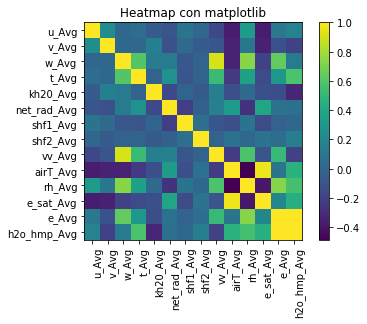
\includegraphics[scale = .7]{matplot.png}
    \caption{Heatmap realizado con la biblioteca de matplotlib}
    \label{fig:matplot}
\end{figure}
\begin{figure}
    \centering
    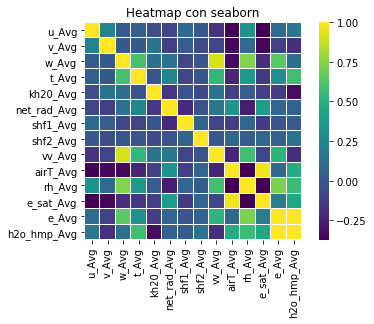
\includegraphics[scale = .7]{seaborn.png}
    \caption{Heatmap realizado con la biblioteca de seaborn}
    \label{fig:seaborn}
\end{figure}
\begin{figure}
    \centering
    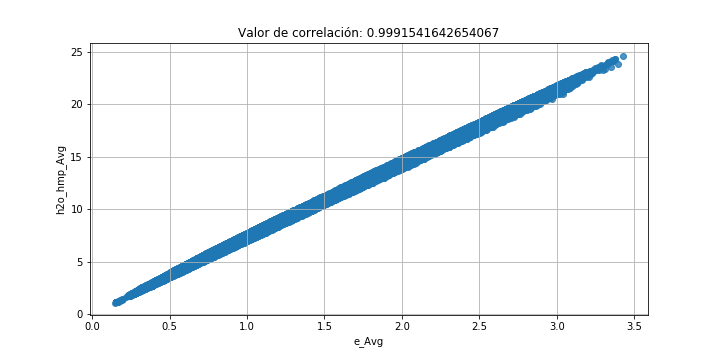
\includegraphics[scale = .53]{evh.png}
    \caption{Gr\'afica de e Avg contra h2o hmp Avg con correlaci\'on lineal de 60.13\%}
    \label{fig:evh2o}
\end{figure}
\begin{figure}
    \centering
    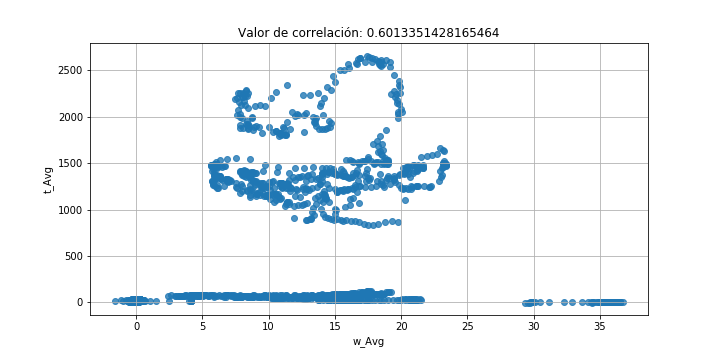
\includegraphics[scale = .53]{wvt.png}
    \caption{Gr\'afica de w Avg contra t Avg con correlaci\'on lineal de 99.91\%}
    \label{fig:wvt}
\end{figure}
\end{document}
